% 2008 年上海卷文科第 17 题：扇形 AOC，出入口在 A、C，内部小路 AD、DC，
%   拐弯处 D 的转角为 120°，CD=500 m，DA=300 m。
% 来源 PDF：gaokaomath-src/普通高考/2008/2008上海文.pdf
% SHA-256：415d384fcd05cab11debea2d8a328f9daf1d1880ffd26c915df999f7bae589a4
% 原页：2008上海文.pdf 第 1 页（A3 三栏）第 3 栏，书页码 481。
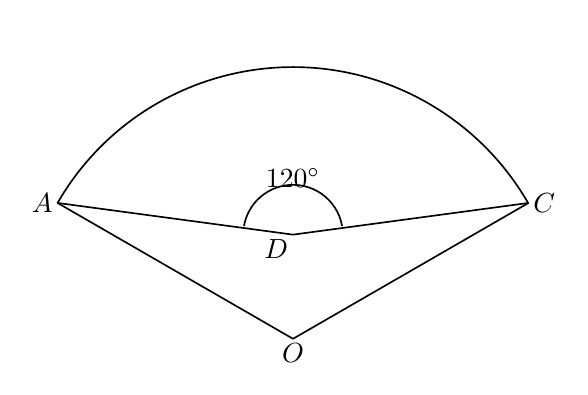
\begin{tikzpicture}[scale=1.15, semithick,
  every node/.style={inner sep=1.5pt}]
  \coordinate (O) at (0,0);
  \coordinate (A) at (-2.6,1.5);
  \coordinate (C) at (2.6,1.5);
  \coordinate (D) at (0,1.15);

  % 扇形弧
  \draw (A) arc[start angle=150, end angle=30, radius=3.0];
  \draw (O) -- (A);
  \draw (O) -- (C);

  % 小路
  \draw (A) -- (D) -- (C);

  % 转角
  \draw (D) ++(10:0.55) arc[start angle=10, end angle=170, radius=0.55];
  \node at (0,1.78) {$120^\circ$};

  \node[left] at (A) {$A$};
  \node[right] at (C) {$C$};
  \node[below left] at (D) {$D$};
  \node[below] at (O) {$O$};
\end{tikzpicture}
